

Useful Linear Algebra tools are matrix factorizations (or decompositions).
They write the matrix $\mat{A}$ as the product of matrices. Special matrices used in the decompositions are triangular and diagonal matrices.

We start by considering factorizations by triangular matrices.

\subsection{Gaussian Elimination Method or LU factorization}

\begin{definition}
    Let $\mat{A} \in \set{R}^{n \times n}$. If $\mat{A}$ is non singular and all the principal submatrices $A_i, i=1 \ldots n-1$ are non singular, then there exists two matrices $\mat{L}$ and $\mat{U}$, with $\mat{L}$ lower triangular with $l_{ii}=1, i=1, \ldots n$ and $\mat{U}$ upper triangular non singular, such that:
    $$ \mat{A} = \mat{L}\mat{U} $$
    We call this an $\mat{LU}$\textit{-factorization} of $\mat{A}$.
\end{definition}

% If $\mat{A}$ is non-singular, so are both $\mat{L}$ and $\mat{U}$ and the solution of the linear system $\mat{A}\vec{x} = \vec{b}$ can be computed by solving two triangular systems
% $$
%     \begin{matrix}
%         \mat{L}\vec{y} = \vec{b}\ \text{(forward substitutions algorithm)}\\
%         \mat{U}\vec{x} = \vec{y}\ \text{(backward substitutions algorithm)}
%     \end{matrix}
% $$

The matrices $\mat{L}$ and $\mat{U}$ can be computed in $n-1$ steps with the so called Gaussian Elimination Method (GEM) having a computational cost of 
$\mathrm{O}(n^{3}/3)$.

% Let $\mat{A}^{(1)} = \mat{A}$ and $k = 1, \hdots, n-1$. 
The matrix $\mat{U}$ can be computed as follows:

\begin{enumerate}
     \item We define $\mat{M}^{(k)}$ the matrix of multipliers with elements
     \begin{itemize}
         \item $m_{ii}=1,\ i = 1, \hdots, n$
         \item $m_{ik} = - \frac{a^{(k)}_{ik}}{a^{(k)}_{kk}},\ i = k + 1, \hdots, n$
        \item $m_{ij} = 0,\ otherwise$
     \end{itemize}
     \item We compute $\mat{A}^{(k+1)} = \mat{M}^{(k)}\mat{A}^{(k)}$
     \item We repeat steps 1-2 until we obtain $\mat{A}^{(n)} = \mat{U}$
 \end{enumerate}

 We therefore have
 $$
     \begin{matrix}
        \mat{M}^{(n-1)}\mat{M}^{(n-2)}\hdots\mat{M}^{(1)}\mat{A} = \mat{U}\\
        \mat{A} = \inv{(\mat{M}^{(n-1)}\mat{M}^{(n-2)}\hdots\mat{M}^{(1)})}\mat{U}\\         \mat{L} = \inv{(\mat{M}^{(n-1)}\mat{M}^{(n-2)}\hdots\mat{M}^{(1)})}
     \end{matrix}
 $$
 
\textbf{Example}
$$
A = 
\begin{pmatrix}
2 & 1 & 0\\
4 & 5 & 2\\
6 & 15 & 12
\end{pmatrix}
\quad
L_1 = 
\begin{pmatrix}
1 & 0 & 0\\
-2 & 1 & 0\\
-3 & 0 & 1
\end{pmatrix}
$$

$$
L_1 \cdot A = A_1 = \begin{pmatrix}
1 & 0 & 0\\
-2 & 1 & 0\\
-3 & 0 & 1
\end{pmatrix} \cdot
\begin{pmatrix}
2 & 1 & 0\\
4 & 5 & 2\\
6 & 15 & 12
\end{pmatrix} = 
\begin{pmatrix}
2 & 1 & 0\\
0 & 3 & 2\\
0 & 12 & 12
\end{pmatrix}
$$

$$
A_1 = 
\begin{pmatrix}
2 & 1 & 0\\
0 & 3 & 2\\
0 & 12 & 12
\end{pmatrix}
\quad
L_2 = 
\begin{pmatrix}
1 & 0 & 0\\
0 & 1 & 0\\
0 & -4 & 1
\end{pmatrix}
$$

$$
L_2 \cdot A_1 = A_2 = 
\begin{pmatrix}
1 & 0 & 0\\
0 & 1 & 0\\
0 & -4 & 1
\end{pmatrix} \cdot
\begin{pmatrix}
2 & 1 & 0\\
0 & 3 & 2\\
0 & 12 & 12
\end{pmatrix} = 
\begin{pmatrix}
2 & 1 & 0\\
0 & 3 & 2\\
0 & 0 & 4
\end{pmatrix} = U
$$
So
$$
L_2L_1A=U \longrightarrow A=L_1^{-1}L_2^{-1}U \longrightarrow L=L_1^{-1}L_2^{-1}=
\begin{pmatrix}
1 & 0 & 0\\
2 & 1 & 0\\
3 & 4 & 1
\end{pmatrix}
$$
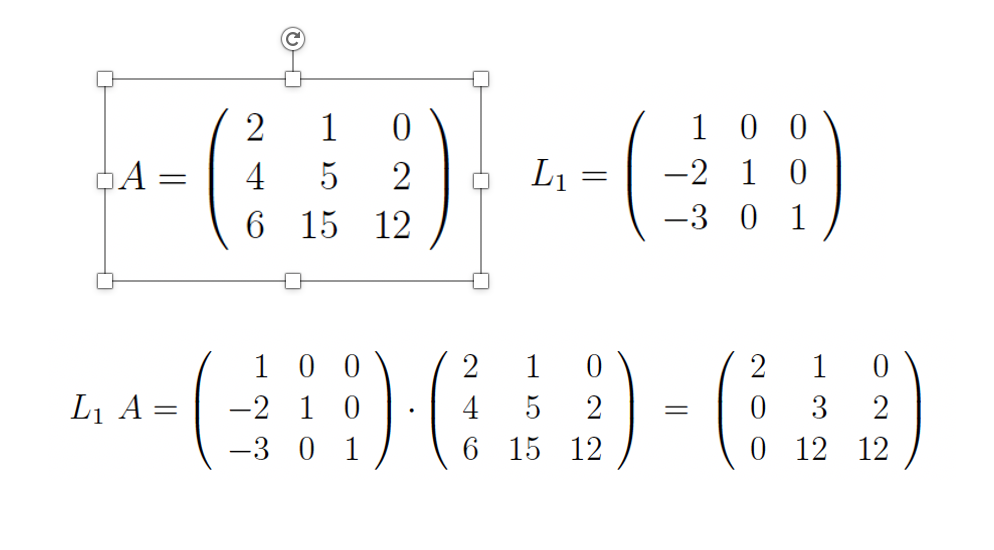
\includegraphics[width=0.7 \textwidth]{sections/lu1.png}

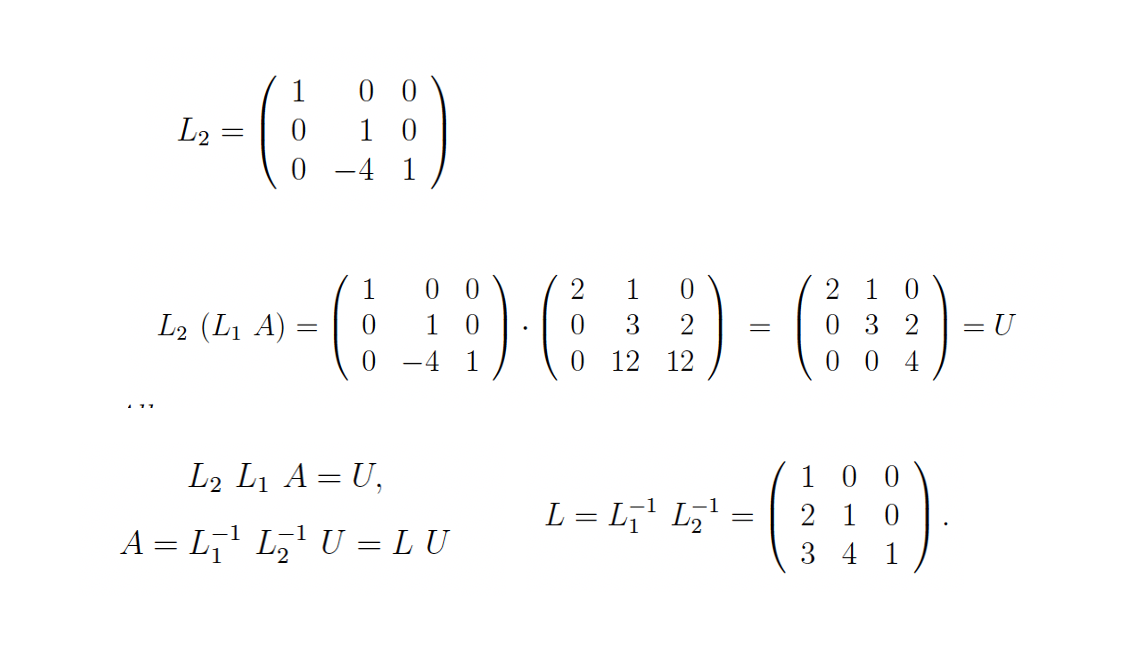
\includegraphics[width=0.8 \textwidth]{sections/lu2.png}

One problem of GEM is that it is \textit{unstable}, i.e. the algorithmic error is not limited. This happens because the elements $a^{(k)}_{kk}$ used to compute the multipliers can be very small or even zero, leading to errors. To avoid this, the \textit{pivoting technique} is employed in order to make the elements $a^{(k)}_{kk}$ as big as possible. This is done by swapping two rows so that $a^{(k)}_{kk}$ is the column element with the maximum absolute value. The swapping can be seen as a left multiplication by a \textit{permutation matrix} $P$, i.e. an identity matrix with the needed rows swapped. 

\textbf{Example}

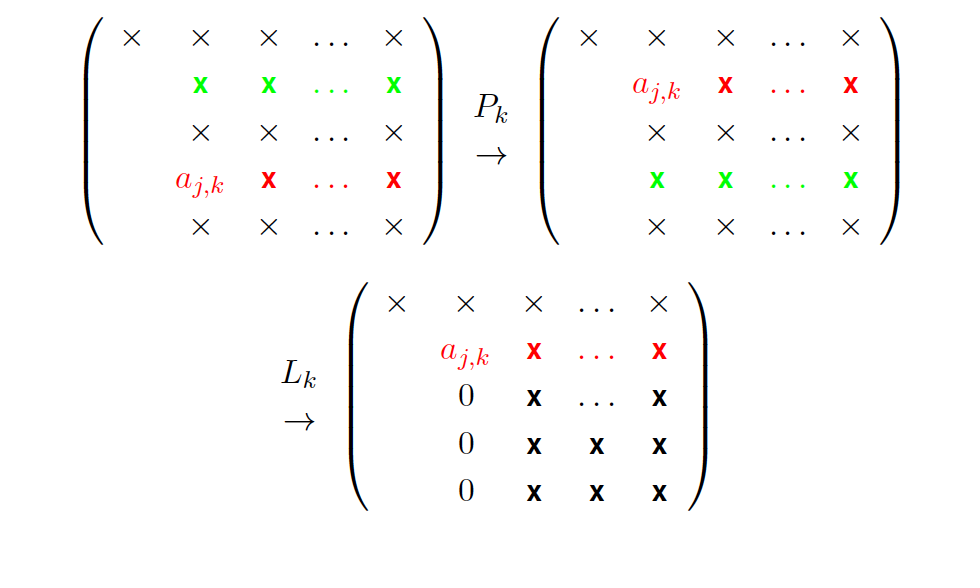
\includegraphics[width=0.7 \textwidth]{sections/images/lup1.png}

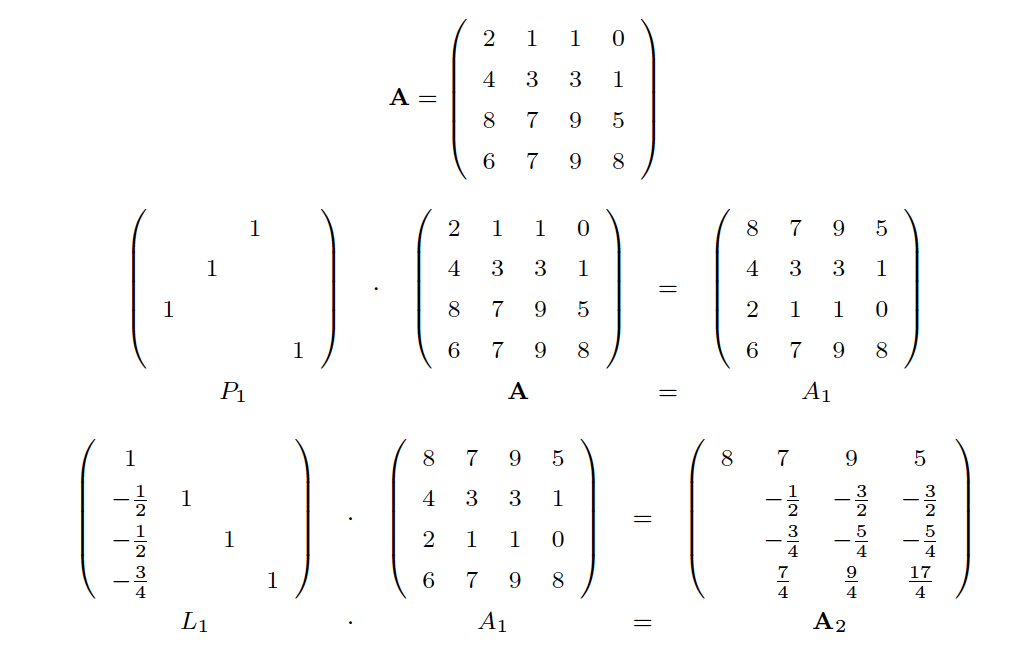
\includegraphics[width=0.8 \textwidth]{sections/images/lup2.png}

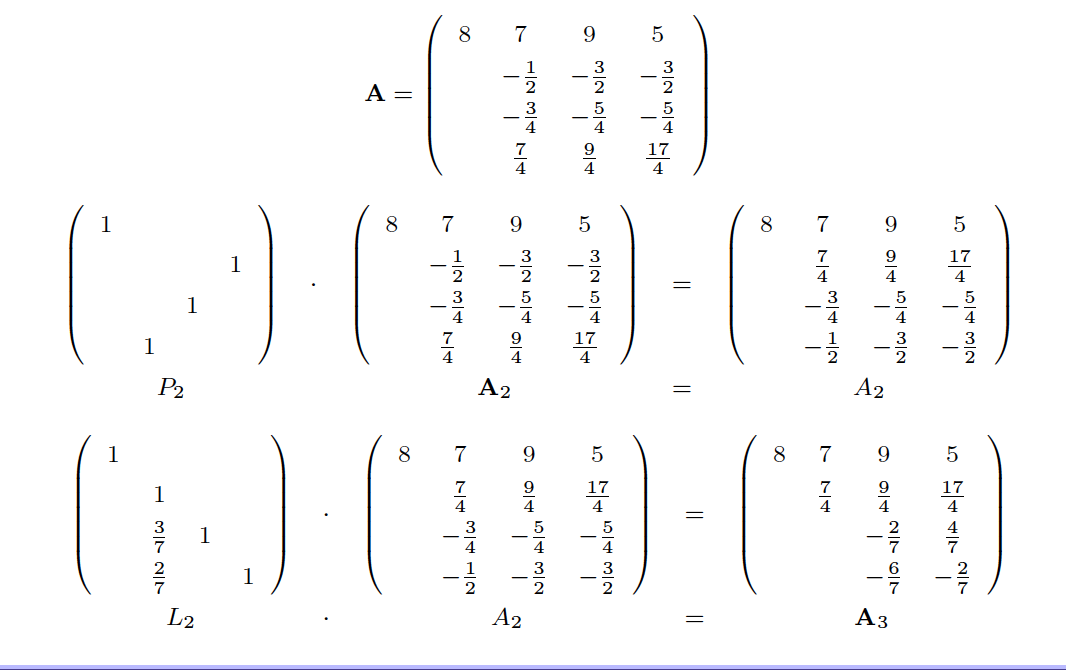
\includegraphics[width=0.8 \textwidth]{sections/images/lup3.png}

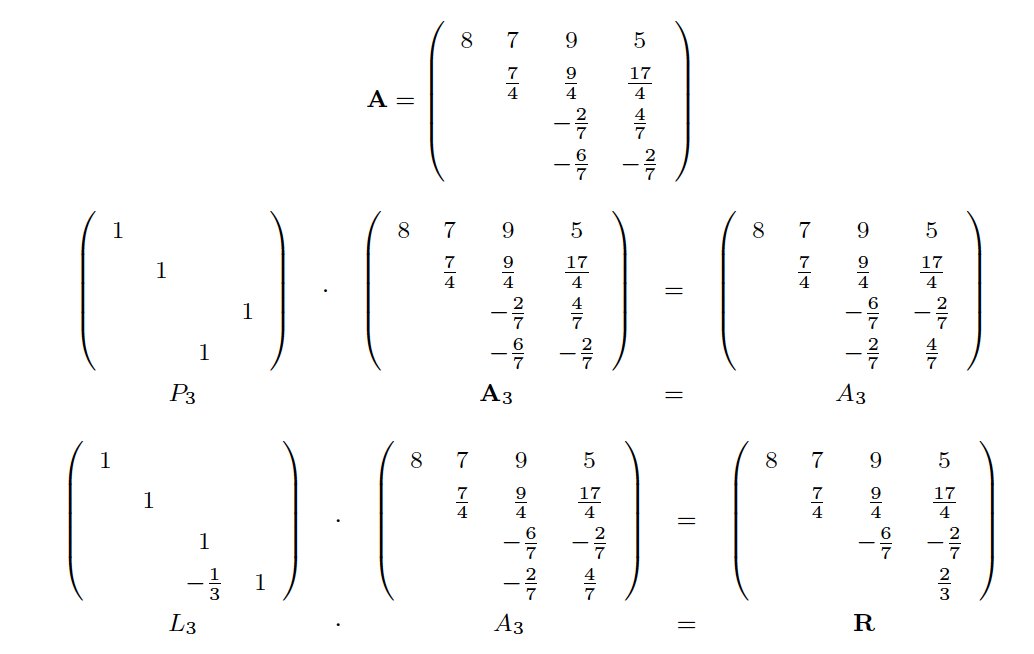
\includegraphics[width=0.8 \textwidth]{sections/images/lup4.png}

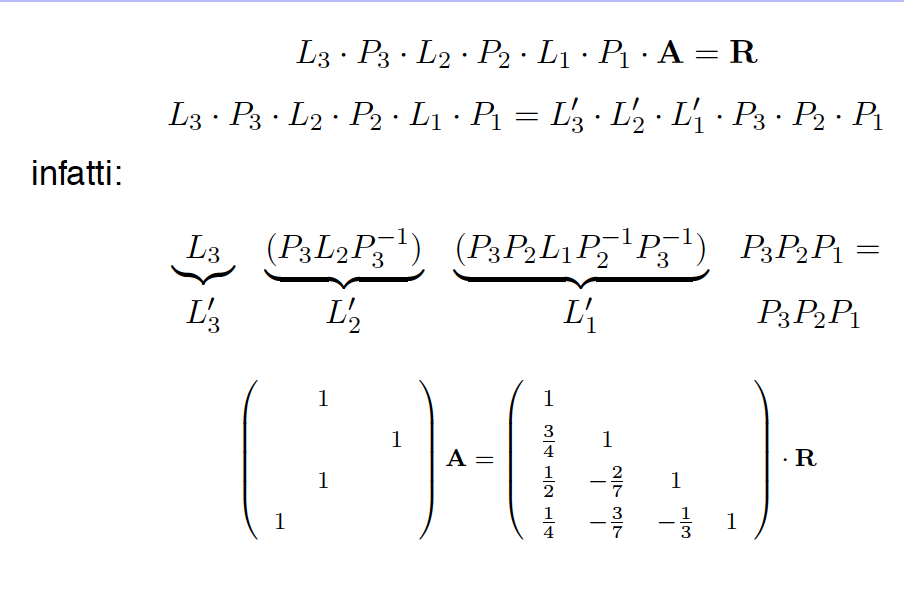
\includegraphics[width=0.8 \textwidth]{sections/images/lup5.png}

% \begin{definition}
%     A matrix $\mat{A} \in \set{R}^{n \times n}$ is positive semi-definite if
%     $$ \forall\vec{x}\in\set{R}^{n},\ \vec{x}\neq\vec{0}\ \ \ \transp{\vec{x}}\mat{A}\vec{x} \geq 0 $$
% \end{definition}

\begin{proposition}
    Let $\mat{A} \in \set{R}^{n \times n}$ be symmetric positive semi-definite. Then it is always possible to $\mat{LU}$-factorize it without using pivoting. In this case we have
    $$ \mat{A} = \mat{L}\transp{L} $$
    
    and the factorization has a computational complexity of $\mathrm{O}(n^3/6)$ (using Cholesky algorithm).
\end{proposition}

\textbf{Example}

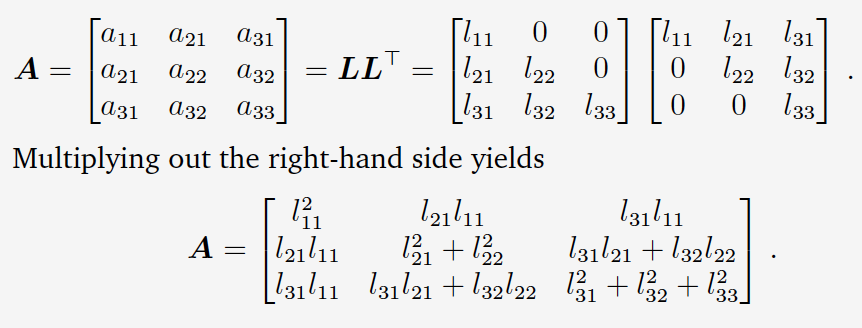
\includegraphics[width=0.7 \textwidth]{sections/images/chol1.png}

The elements $l_{ij}$ of the matrix $\mat{L}$ are computed by comparing the left and roght hand sides of the previous matrix equation.

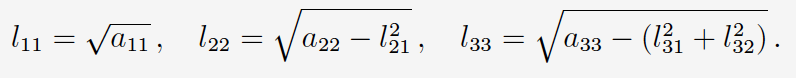
\includegraphics[width=0.8 \textwidth]{sections/images/chol2.png}

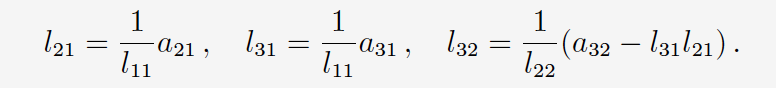
\includegraphics[width=0.8 \textwidth]{sections/images/chol3.png}

The Cholesky decomposition is a very useful tool in numerical linear algebra for Machine Learning, where we often encounter symmetric positive definite matrices. For example, the covariance matrix of a multivariate Gaussian variable
is symmetric positive definite. \\
Moreover, the Cholesky decomposition can be used to efficiently compute the determinant of a symmetric positive definite matrix. We know that $$det(\mat{A})=det(\mat{L}) det(\mat{L^T})=det(\mat{L}^2)=\prod_i l_{ii}^2.$$

\subsection{Singular Value Decomposition (SVD)}

We introduce here a decomposition that involve a diagonal matrix instead of Triangular matrices.

There are mainly two matrix decompositions involving a diagonal matrix: the so called \textit{eigendecomposition} and the \textit{Singular Value Decomposition}.
We will go quickly through the first one and we will analyse in detail the second.

\begin{proposition}
\textit{Eigendecomposition.} Let $\mat{A}$ a square matrix of size $n \times n$. Hence $\mat{A}$ A can be decomnposed as:
$$\mat{A}=\mat{PDP}^{-1}$$
where $\mat{P}$ is a non singular matrix of size $n \times n$ and $\mat{D}$ is a diagonal matrix with diagonal elements $d_{ii}$ corresponding to the eigenvalues of $\mat{A}$ iff the eigenvectors of $\mat{A}$ are linear independent abd form a basis of $]\mathbf{R}^n$.
\end{proposition}

Example 4.11 MML book.

\textbf{Observation.} The eigenvalue decomposition can be applied only to square matrices and with particular properties on their spectrum.

We now introduce the Singulas Value Decomposition (SVD) which can be applied to \textbf{all} the matrices.
We first need some definitions and concepts on \textit{orthogonality}. 

\begin{definition}
    Let $\vec{u}, \vec{v} \in \set{R}^n$. $\vec{u}$ and $\vec{v}$ are \textit{orthogonal} if
    $$ \langle\vec{u}, \vec{v}\rangle = 0 $$
\end{definition}

\begin{definition}
    $\vec{u} \in \set{R}^n$ is a \textit{unit vector} if $\norm{\vec{u}} = 1$.
\end{definition}

\begin{proposition}
    (Normalization) $\forall\vec{u} \in \set{R}^n,\ \ \ \hat{\vec{u}} = \frac{\vec{u}}{\norm{\vec{u}}}$ is a unit vector.
\end{proposition}

\begin{example}
    $$ \vec{u} = [1, 2, 3] $$
    $$ \norm{\vec{u}}_2 = \sqrt{14} $$
    $$ \hat{\vec{u}} = \frac{\vec{u}}{\norm{\vec{u}}} = \left[ \frac{1}{\sqrt{14}}, \frac{2}{\sqrt{14}}, \frac{3}{\sqrt{14}} \right] $$
\end{example}

\begin{definition}
    The set $\{\vec{u}_1, \vec{u}_2, \hdots, \vec{u}_p\},\ \vec{u}_i \in \set{R}^n,\ i = 1, \hdots, p$ is an \textit{orthogonal set} if $\langle\vec{u}_i, \vec{u}_j\rangle = \transp{\vec{u}_i}\vec{u}_j = 0,\ \forall i \neq j$
\end{definition}

\begin{example}
    $$ \vec{u}_1 = \transp{[3, 1, 1]},\ \vec{u}_2 = \transp{[-1, 2, 1]},\ \vec{u}_3 = \transp{\left[ -\frac{1}{2}, -2, \frac{7}{2} \right]} $$
    is an orthogonal set because
    $$ \langle\vec{u}_1, \vec{u}_2\rangle = 0,\ \langle\vec{u}_1, \vec{u}_3\rangle = 0,\ \langle\vec{u}_2, \vec{u}_3\rangle = 0,\  $$
\end{example}

\begin{proposition}
    If $\vec{u}_1, \vec{u}_2, \hdots, \vec{u}_p \in \set{R}^n$ are orthogonal then they are linearly independent. The set $\{\vec{u}_1, \vec{u}_2, \hdots, \vec{u}_p\},\ \vec{u}_i \in \set{R}^n,\ i = 1, \hdots, p$ is an \textit{orthogonal basis} for $U = \text{span}\{\vec{u}_1, \vec{u}_2, \hdots, \vec{u}_p\}$.
\end{proposition}

\begin{definition}
    The set $\{\vec{u}_1, \vec{u}_2, \hdots, \vec{u}_p\},\ \vec{u}_i \in \set{R}^n,\ i = 1, \hdots, p$ is an \textit{orthonormal set} if it is an orthogonal set of unit vectors. A basis of orthonormal vectors is called \textit{orthonormal basis}.
\end{definition}

\begin{definition}
    Let $\mat{U} \in \set{R}^{m \times n}$. $\mat{U}$ is an \textit{orthogonal matrix} iff $\transp{U}\mat{U} = \mat{I}$. If $m = n$ then $\transp{U} = \inv{U}$.
\end{definition}

\begin{proposition}
    If $\mat{U}^{m \times n}$ is orthogonal then
    
    \begin{itemize}
        \item $\norm{\mat{U}\vec{x}}_2 = \norm{\vec{x}}_2,\ \forall\vec{x} \in \set{R}^n$
        \item $\langle\mat{U}\vec{x}, \mat{U}\vec{y}\rangle = \langle\vec{x}, \vec{y}\rangle,\ \forall\vec{x}, \vec{y} \in \set{R}^n$
        \item $\langle\mat{U}\vec{x}, \mat{U}\vec{y}\rangle = 0 \iff \langle\vec{x}, \vec{y}\rangle = 0,\ \forall\vec{x}, \vec{y} \in \set{R}^n$
    \end{itemize}
\end{proposition}

Transformations by orthogonal matrices preserve both length and angles.

We present the SVD in the case $m ]\geq n$ but it can be easily extended to the case $m<n$ (see for example MML book).
\begin{proposition}
\textit{singular value decomposition} (SVD).
Any matrix $\mat{A} \in \set{R}^{m \times n},\ m \geq n$ with $\rank{A} = k,\ k \leq n$ can be written as
$$ \mat{A} = \mat{U}\mat{\Sigma}\transp{V} $$
where
\begin{itemize}
    \item $\mat{U} \in \set{R}^{m \times m}$ is an orthogonal matrix with orthogonal vectors $\vec{u}_i$
    \item $\mat{V} \in \set{R}^{n \times n}$ is an orthogonal matrix with orthogonal vectors $\vec{v}_i$
    \item $\Sigma \in \set{R}^{m \times n}$ is a matrix whose diagonal entries are the \textit{singular values} $\sigma_i$ of $\mat{A}$ and with extra-diagonal entries equal to 0.
\end{itemize}
\end{proposition}

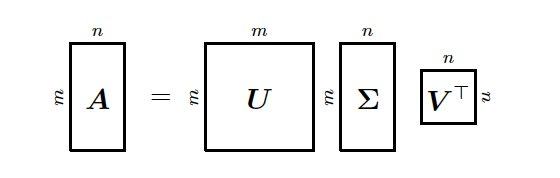
\includegraphics[width=0.7 \textwidth]{sections/images/svd.png}

 The singular values enjoy the following property
    $$ \sigma_1 \geq \sigma_2 \geq \hdots \geq \sigma_k > \sigma_{k+1} = \sigma_{k+2} = \hdots = \sigma_{n} = 0 $$
    where $k = \rank{A}$. The singular matrix $\Sigma$ is unique, while the orthogonal matrices $\mat{U}$ and $\mat{V}$ aren't.

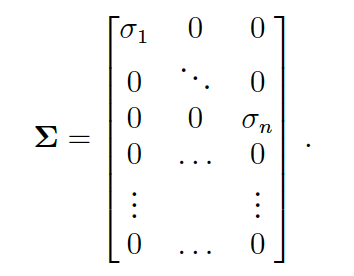
\includegraphics[width=0.5 \textwidth]{sections/images/svd1.png}

From the geometric point of view, the SVD performs two changes of basis, via the orthogonal matrices $\mat{U}$ and $\mat{V}$ and a scaling operation via the matrix $\Sigma$. The columns of $\mat{U}$ and $\mat{V}$ are sets of orthonormal basis of $\mathbf{R}^m$ and $\mathbf{R}^n$, respectively. See Example 4.12 MML book, page 121.

\textit{Results}
\begin{itemize}
\item Since the following relation holds:
$$\mat{A}\vec{v}_i=\sigma_i \vec{u}_i,\ i = 1, \ldots, n$$
$\vec{v}_i$ are called \textit{right singular vectors} and $\vec{u}_i$ are called \textit{left singular vectors}.
\item 
We have the following relation between the singular values of $\mat{A}$ and the eigenvalues of $\mat{A^T A}$.
$$\mat{A^T A}=(\mat{U \Sigma V^T})^T(\mat{U \Sigma V^T})=\mat{V \Sigma ^T U^T U \Sigma V^T}$$
Hence 
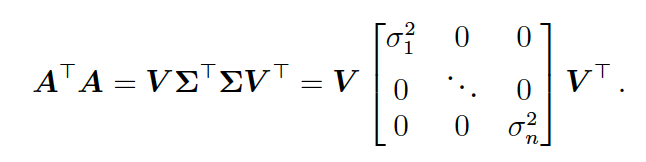
\includegraphics[width=0.7 \textwidth]{sections/images/svd2.png}

and
$$\sigma_i = \sqrt{\lambda_i(\transp{A}\mat{A})},\ i = 1, \hdots, n$$
In particular:
$$ \sigma_1 = \sqrt{\lambda_{max}(\transp{A}\mat{A})} = \sqrt{\rho(\transp{A}\mat{A})} = \norm{A}_2 $$
$$ \sigma_n = \sqrt{\lambda_{min}(\transp{A}\mat{A})} \implies \norm{\inv{A}}_2 = \frac{1}{\sigma_n} $$
Thus,
$$ K(\mat{A}) = \frac{\sigma_1}{\sigma_2} $$
\item The right singular vectors of $\mat{A}$ are the eigenvectors of $\mat{A^T A}$
\item The left singular vectors of $\mat{A}$ are the eigenvectors of $\mat{AA^T }$
\item For symmetric matrices $\mat{A}$ the eigenvalue decomposition and the SVD are one and the same.

\end{itemize}

\textit{Moore-Penrose inverse}.
The SVD can be used to compute the \textit{Moore-Penrose inverse} (or simply \textit{pseudoinverse}) of a matrix $\mat{A} \in \set{R}^{m \times n}$
$$ \mat{A}^{+} = \mat{V}\Sigma^{+}\transp{U} $$
where $\Sigma^{+} \in \set{R}^{n \times m}$ is the pseudoinverse of $\Sigma$, computed by taking the reciprocal of every non-zero diagonal element, leaving the zeros in place and transposing the matrix
$$
    \Sigma =
    \begin{bmatrix}
        \sigma_1 & 0 & \hdots & 0\\
        0 & \sigma_2 & \hdots & 0\\
        0 & 0 & \ddots & 0\\
        0 & 0 & 0 & \sigma_n\\
        0 & 0 & 0 & 0\\
        \vdots & \vdots & \vdots & \vdots\\
        0 & 0 & 0 & 0
    \end{bmatrix},\ \ \ \ 
    \Sigma^{+} =
    \begin{bmatrix}
        \frac{1}{\sigma_1} & 0 & \hdots & 0 & \hdots & 0\\
        0 & \frac{1}{\sigma_2} & \hdots & 0 & \hdots & 0\\
        0 & 0 & \ddots & 0 & \hdots & 0\\
        0 & 0 & 0 & \frac{1}{\sigma_n} & \hdots & 0\\
    \end{bmatrix}
$$


\subsection{Matrix approximation using SVD}
Given the SVD of a matrix $\mat{A} \in \set{R}^{m \times n}$
$$ \mat{A} = \mat{U}\Sigma\transp{V} $$
we can use it to represent (or approximate) the matrix $\mat{A}$ as a sum of low-rank matrices $\mat{A}_i \in \set{R}^{m \times n}$ with $\text{rank}(\mat{A}_i) = 1$ such that
$$ \mat{A}_i = \vec{u}_i\transp{\vec{v}_i} $$
The matrix $ \mat{A}$ of $\rank{A} = k$ can then be written as
$$ \mat{A} = \sum^{k}_{i = 1}{\sigma_i\mat{A}_i} = \sum^{k}_{i = 1}{\sigma_i\vec{u}_i\transp{\vec{v}_i}} $$

To obtain a rank-$p$ approximation $\mat{A}_p$ ($p < k$) of $\mat{A}$ we can truncate the sum at index $i = p$. The error introduced with this approximation can be computed as
$$ \norm{\mat{A} - \mat{A}_p}_2 = \left|\left|\sum^{k}_{i = p+1}{\sigma_i\mat{A}_i}\right|\right|_2 = \sigma_{p+1}$$
This means that if $\sigma_{p+1}$ is small we have a good approximation of the original matrix $\mat{A}$.

\begin{theorem}
    Given $\mat{A} \in \set{R}^{m \times n},\ \rank{A} = k$, let $\mat{A} = \mat{U}\Sigma\transp{V}$ be its singular value decomposition. Let $\mat{A}_p = \sum^{p}_{i = 1}{\sigma_i\vec{u}_i\transp{\vec{v}_i}}$ be the rank-$p$ approximation of $\mat{A}$. Then
    $$ \forall \mat{B} \in \set{R}^{m \times n},\ \rank{B} = p,\ \norm{\mat{A} - \mat{A}_p}_2 \leq \norm{\mat{A} - \mat{B}}_2 $$
    So $\mat{A}_p$ is the best rank-$p$ approximation of $\mat{A}$ obtained via singular value decomposition.
\end{theorem}

Example. \textit{Rank-p approximation of an image matrix}.

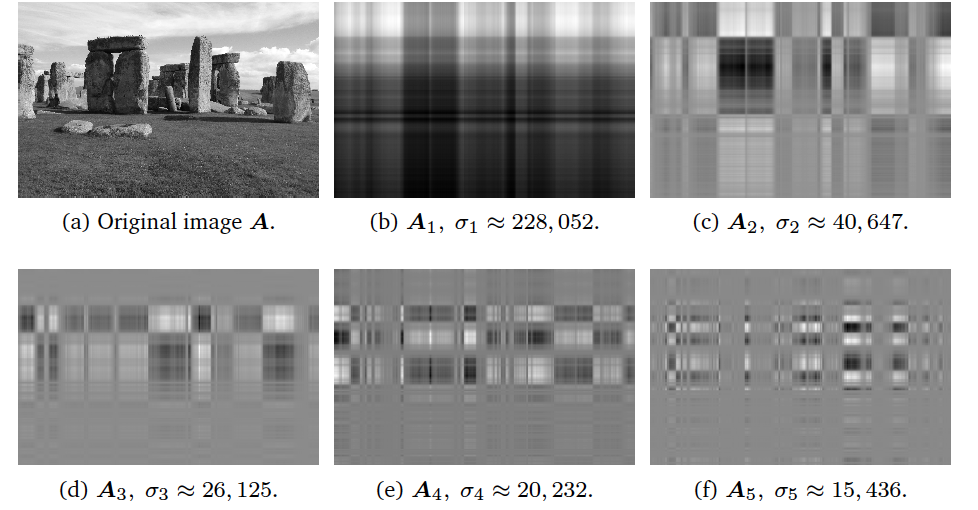
\includegraphics[width=0.7 \textwidth]{sections/images/svd3.png}

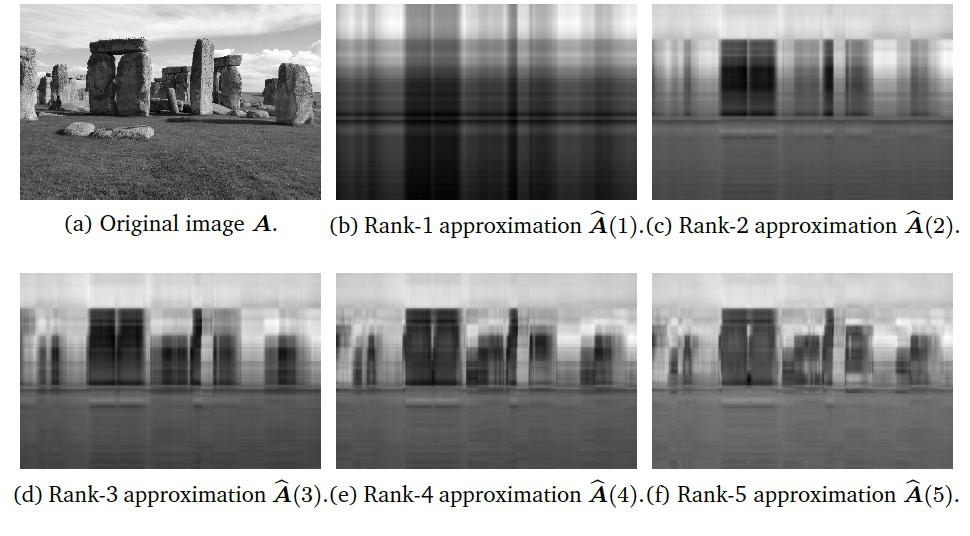
\includegraphics[width=0.7 \textwidth]{sections/images/svd4.png}

The matrix associated to the original image has size $m \times n=1432 \times 1910$, hence it requires 2735120 data. If we consider the rank-p approximation ,it requires $(m+n+1)\times p$ data. For example, the rank-5 approximation requires $5\times(1432+1910+1)=16715$ data, corresponding to about $0.6 \%$ of the original one.
Hence we can interpret the rank-p SVD approximation of a matrix $\mat{A}$ as a lossy compression. This approximation appears in different machine learning applications, such as image processing, noise filtering and regularization of ill-posed problems. Moreover, it is a fundamental tool in the PCA analysis.

We can see the rank-p approximation obtain through SVD as the projection of $\mat{A}$ onto a subspace of matrices of rank p. Among all the possible projections, rank-p SVD approximation minimizes the error in the 2-norm betweeen $\mat{A}$ and any rank-p approximation of $\mat{A}$.

Examples 4.14 and 4.15 MML book \textit{finding structure in Movie Ratings and Customers}

\subsection{Conclusions}

We can summarize many tools and ideas in the following figure, where we can see the relationship between different types of matrices.

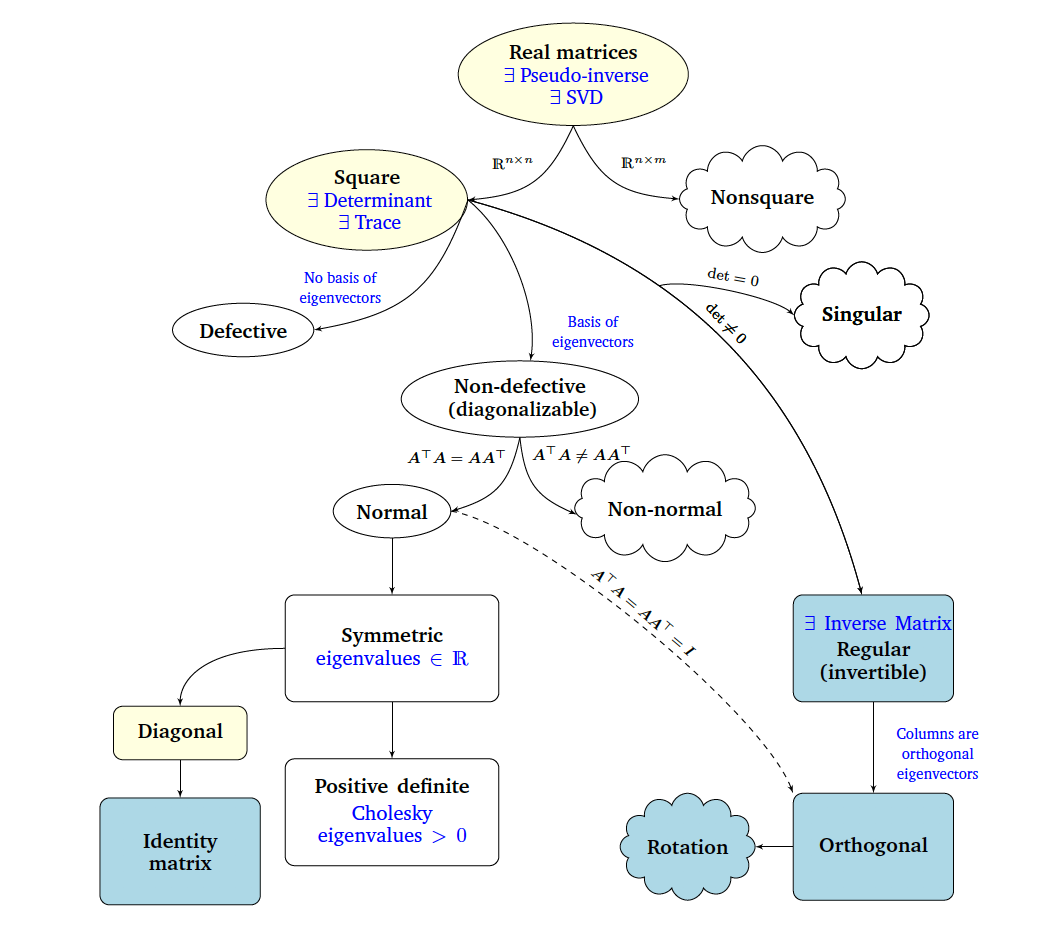
\includegraphics[width=0.7 \textwidth]{sections/images/matrix.png}